\documentclass{article}
\usepackage{graphicx}
\usepackage{hyperref}
\usepackage{enumitem}
\usepackage{datetime}
\usepackage{textcomp}

\usepackage{xcolor}


\begin{document}

\begin{tabular}{@{}ll}
    \textbf{\huge Hanxiao Liu} \newline
    \includegraphics*[draft,natwidth=90, natheight=36]{img/name-cn.png}
    \HCode{<script type="text/javascript" src="email.js"></script>} \newline
    6227 Gates-Hillman Center \ \ \newline
    Carnegie Mellon University
    &
    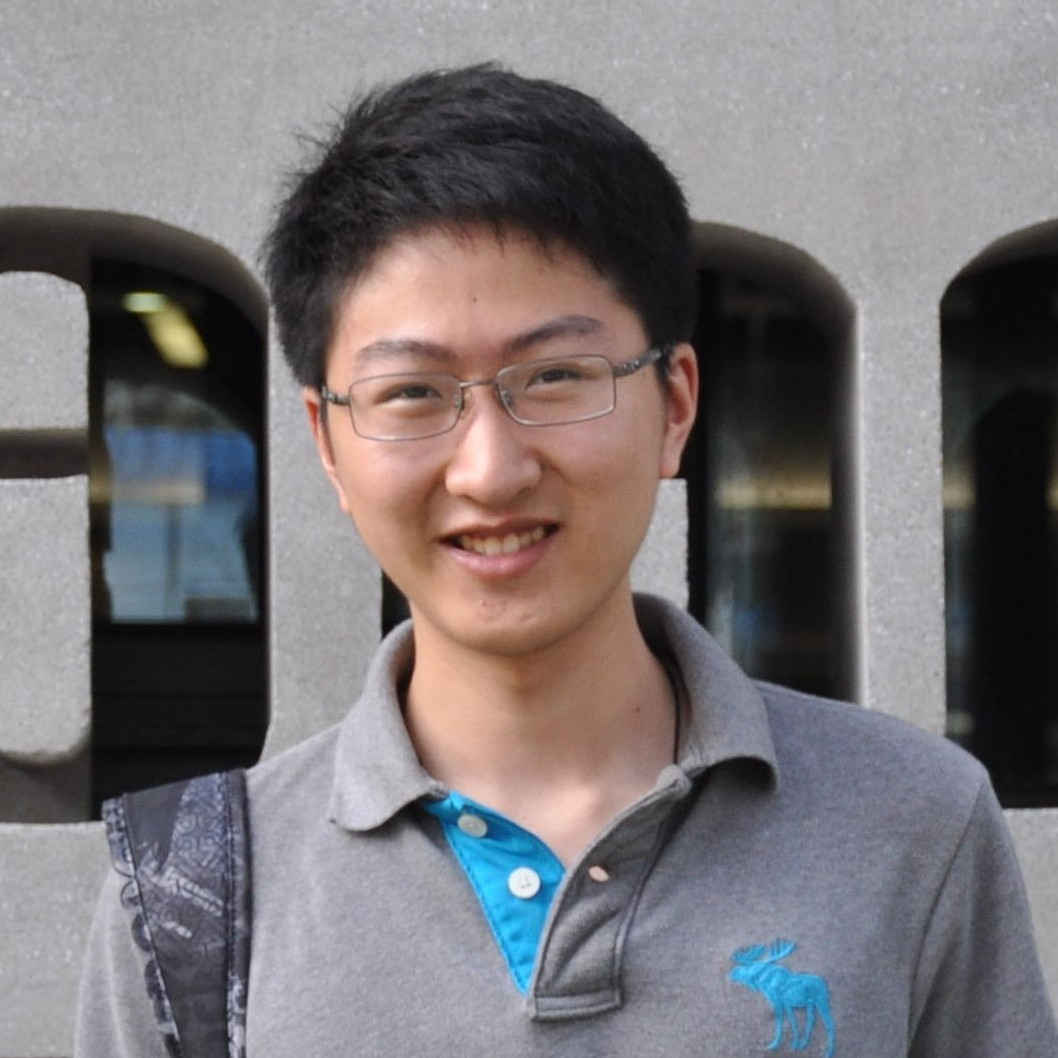
\includegraphics[natwidth=121, natheight=121]{img/profile.jpg} \\
\end{tabular}


\subsection*{Readme}
I have joined \href{https://ai.google/research/teams/brain}{Google Brain} as a research scientist.

\noindent I received my Ph.D. from the 
\href{http://www.lti.cs.cmu.edu/}{Language Technologies Institute},
\href{http://www.scs.cmu.edu/}{School of Computer Science} at
\href{http://www.cmu.edu/index.shtml}{Carnegie Mellon University} in 2018,
working with Professor \href{http://www.cs.cmu.edu/~./yiming/}{Yiming Yang}.
Prior to that,
I received my B.E.\ from Department of Automation at
\href{http://www.tsinghua.edu.cn/publish/newthuen/index.html}{Tsinghua University} in 2013.

\noindent
My research interests include deep learning, meta-learning and language understanding.
Recently, I'm working on the automatic design of neural architectures.


\subsection*{Work Experience}
\begin{itemize}
	\item \emph{Research Intern}, \href{https://deepmind.com/}{DeepMind}, London, Summer 2017. \\
		Neural architecture search for image recognition, with \href{http://www.robots.ox.ac.uk/~karen/}{Karen Simonyan}.
	\item \emph{Quantitative Research Intern}, \href{https://www.citadel.com/}{Citadel LLC}, Chicago, Summer 2016. \\
		Statistical arbitrage and high-frequency trading.
	\item \emph{Research Intern}, \href{http://research.microsoft.com/en-us/labs/asia/}{Microsoft Research Asia}, Beijing, Spring 2013. \\
		Game theory in computational advertising,
		with \href{https://www.microsoft.com/en-us/research/people/wche/}{Wei Chen},
		\href{https://www.microsoft.com/en-us/research/people/taoqin/}{Tao Qin} and \href{https://www.microsoft.com/en-us/research/people/tyliu/}{Tie-Yan Liu}.
\end{itemize}


\subsection*{Publications
	\ \ \ \ --- \protect
\href{https://github.com/quark0}{
\includegraphics[natwidth=20, natheight=20]{img/GitHub-Mark-64px.png}}
\href{https://scholar.google.com/citations?user=IMkVH_8AAAAJ&hl=en}{
\includegraphics[natwidth=20, natheight=20]{img/google-scholar.png}}
---
}
\begin{itemize}
	\item 
		\href{https://arxiv.org/abs/1806.09055}{DARTS: Differentiable Architecture Search}
		\
		\texttt{\scriptsize |\href{https://github.com/quark0/darts}{Code}|} \\
		\emph{Hanxiao Liu}, Karen Simonyan, Yiming Yang. \\
		\textbf{ICLR 2019}.
	\item
		\href{https://arxiv.org/pdf/1703.07015.pdf}{Modeling Long- and Short-Term Temporal Patterns with Deep Neural Networks}
		\
		\texttt{\scriptsize |\href{https://github.com/laiguokun/LSTNet}{Code}|} \\
		Guokun Lai, Wei-Cheng Chang, Yiming Yang, \emph{Hanxiao Liu}. \\
		\textbf{SIGIR 2018}.
	\item 
		\href{https://arxiv.org/abs/1711.00436}{Hierarchical Representations for Efficient Architecture Search} \\
		\emph{Hanxiao Liu}, Karen Simonyan, Oriol Vinyals, Chrisantha Fernando, Koray Kavukcuoglu. \\
		\textbf{ICLR 2018}. \\
	\item 
		\href{https://arxiv.org/abs/1704.04683}{RACE: Large-Scale Reading Comprehension Dataset from Examinations}
		\
		\texttt{\scriptsize |\href{http://www.cs.cmu.edu/~glai1/data/race/}{Data},\href{http://www.qizhexie.com/data/RACE_leaderboard}{Leaderboard}|} \\
		Guokun Lai, Qizhe Xie, \emph{Hanxiao Liu}, Yiming Yang, Eduard Hovy. \\
		\textbf{EMNLP 2017}.
	\item 
		\href{https://arxiv.org/abs/1705.02426}{Analogical Inference for Multi-Relational Embeddings}
		\
		\texttt{\scriptsize |\href{slides/icml2017-liu.pdf}{Slides},\href{https://github.com/quark0/ANALOGY}{Code}|} \\
		\emph{Hanxiao Liu}, Yuexin Wu, Yiming Yang. \\
		\textbf{ICML 2017}.
	\item 
		\href{http://arxiv.org/abs/1606.01549}{Gated-Attention Readers for Text Comprehension}
		\
		\texttt{\scriptsize |\href{https://github.com/bdhingra/ga-reader}{Code}|}
		\\
		Bhuwan Dhingra*, \emph{Hanxiao Liu}*, Zhilin Yang, William W. Cohen, Ruslan Salakhutdinov. \\
		\textbf{ACL 2017}.
	\item
		\href{publications/chang-wu-aaai17.pdf}{Cross-Domain Kernel Induction for Transfer Learning} \\
		Wei-Cheng Chang, Yuexin Wu, \emph{Hanxiao Liu}, Yiming Yang. \\
		\textbf{AAAI 2017}.
	\item
		\href{publications/murugesan-liu-nips16.pdf}{Adaptive Smoothed Online Multi-Task Learning} \\
		\emph{Hanxiao Liu}*, Keerthiram Murugesan*, Jaime G. Carbonell, Yiming Yang. \\
		\textbf{NeurIPS 2016}.
	\item
		\href{publications/xu-cikm16.pdf}{Cross-Lingual Text Classification via Model Translation with Limited Dictionaries} \\
		Ruochen Xu, Yiming Yang, \emph{Hanxiao Liu}, Andrew Hsi. \\
		\textbf{CIKM 2016}. 
	\item 
		\href{publications/liu-icml16.pdf}{Cross-Graph Learning of Multi-Relational Associations}
		\
		\texttt{\scriptsize |\href{slides/icml2016-liu.pdf}{Slides}|} \\
		\emph{Hanxiao Liu} and Yiming Yang. \\
		\textbf{ICML 2016}.
	\item
		\href{publications/liu-aistats16.pdf}{Semi-Supervised Learning with Adaptive Spectral Transform} \\
		\emph{Hanxiao Liu} and Yiming Yang. \\
		\textbf{AISTATS 2016}.
	\item
		\href{publications/liu-jair16.pdf}{Learning Concept Graphs from Online Educational Data}
		\
		\texttt{\scriptsize |\href{https://github.com/quark0/CGL}{Code}|} \\
		\emph{Hanxiao Liu}, Wanli Ma, Yiming Yang, Jaime G. Carbonell. \\
		\textbf{Journal of AI Research}.
	\item 
		\href{publications/liu-icml15.pdf}{Bipartite Edge Prediction via Transductive Learning over Product Graphs}
		\
		\texttt{\scriptsize |\href{slides/icml2015-liu.pdf}{Slides},\href{publications/liu-icml15-supp.pdf}{Supp}|} \\
		\emph{Hanxiao Liu} and Yiming Yang. \\
		\textbf{ICML 2015}. \\
	\item
		\href{publications/yang-wsdm15.pdf}{Concept Graph Learning from Educational Data}
		\
		\texttt{\scriptsize |\href{slides/wsdm2015-liu.pdf}{Talk},\href{https://github.com/quark0/CGL}{Code}|} \\
		Yiming Yang, \emph{Hanxiao Liu}, Jaime G. Carbonell, Wanli Ma. \\
		\textbf{WSDM 2015}. \\
\end{itemize}
{\textit{``*'' indicates equal contribution. Co-first authors are ordered alphabetically.}}

%\subsection*{Technical Reports}
%\begin{itemize}
%\item \href{https://arxiv.org/abs/1710.11577}{Learning Graph Convolution Filters from Data Manifold}
	%\
	%\texttt{\scriptsize |\href{https://github.com/laiguokun/DSGC}{Code}|} \\
	%Guokun Lai, \emph{Hanxiao Liu}, Yiming Yang. \\
	%\emph{arXiv:1710.11577}. \\
    %\item
	%\href{https://arxiv.org/abs/1703.00993}{A Comparative Study of Word Embeddings for Reading Comprehension} \\
	%Bhuwan Dhingra, \emph{Hanxiao Liu}, Ruslan Salakhutdinov, William W. Cohen. \\
	%\emph{arXiv:1703.00993}.
%\end{itemize}


\subsection*{Professional Activities}
Reviewer, \emph{International Conference on Machine Learning} (ICML), 2016, 2017, 2018, 2019. \\
Reviewer, \emph{Neural Information Processing Systems} (NeurIPS), 2016, 2017, 2018. \\
Reviewer, \emph{International Conference on Learning Representations} (ICLR), 2019. \\
Reviewer, \emph{AAAI Conference on Artificial Intelligence} (AAAI), 2017, 2018, 2019. \\
Reviewer, \emph{Journal of Machine Learning Research} (JMLR). \\
Reviewer, \emph{Neural Computation}.


\subsection*{Notes \& Lectures}
\begin{enumerate}
	\item \href{slides/rl.pdf}{Reinforcement Learning, Basics}
	\item \href{slides/rl-po.pdf}{Reinforcement Learning, Policy Optimization}
	\item \href{slides/adversarial.pdf}{Adversarial Examples}
	\item \href{slides/rademacher_vc_hanxiaol.pdf}{Rademacher Complexity and VC Dimension}
	\item \href{slides/gan.pdf}{Generative Adversarial Networks}
	\item \href{slides/sp.pdf}{Spectral Analysis of Stationary Stochastic Process}
	\item \href{slides/screening.pdf}{Screening Tests for the Lasso}
	\item \href{slides/hanxiaol-sgd.pdf}{Large-Scale Stochastic Optimization}
	\item \href{slides/hanxiaol-adagrad.pdf}{Adaptive Stochastic Subgradient Methods}
	\item \href{slides/hanxiaol-bvmf.pdf}{Variational Inference for Bayes von Mises-Fisher Mixture}
	\item \href{slides/hanxiaol-emvb.pdf}{The EM algorithm and Variational Bayes}
	\item \href{slides/spectral_learning.pdf}{Spectral Algorithms}
\end{enumerate}


\subsection*{}
\footnotesize{
    \textit{
        Last compiled on \today\ by \href{http://www.tug.org/tex4ht/}{\TeX4ht}. \newline
        Copyright \textcopyright\ \the\year\ Hanxiao Liu. All Rights Reserved.
    }
}

\end{document}
